\PassOptionsToPackage{unicode=true}{hyperref} % options for packages loaded elsewhere
\PassOptionsToPackage{hyphens}{url}
\PassOptionsToPackage{dvipsnames,svgnames*,x11names*}{xcolor}
%
\documentclass[12pt,a4paper]{article}
\usepackage{lmodern}
\usepackage{amssymb,amsmath}
\usepackage{ifxetex,ifluatex}
\usepackage{fixltx2e} % provides \textsubscript
\ifnum 0\ifxetex 1\fi\ifluatex 1\fi=0 % if pdftex
  \usepackage[T1]{fontenc}
  \usepackage[utf8]{inputenc}
  \usepackage{textcomp} % provides euro and other symbols
\else % if luatex or xelatex
  \usepackage{unicode-math}
  \defaultfontfeatures{Ligatures=TeX,Scale=MatchLowercase}
\fi
% use upquote if available, for straight quotes in verbatim environments
\IfFileExists{upquote.sty}{\usepackage{upquote}}{}
% use microtype if available
\IfFileExists{microtype.sty}{%
\usepackage[]{microtype}
\UseMicrotypeSet[protrusion]{basicmath} % disable protrusion for tt fonts
}{}
\IfFileExists{parskip.sty}{%
\usepackage{parskip}
}{% else
\setlength{\parindent}{0pt}
\setlength{\parskip}{6pt plus 2pt minus 1pt}
}
\usepackage{xcolor}
\usepackage{hyperref}
\hypersetup{
            pdfauthor={Mark Myatt and Ernest Guevarra},
            colorlinks=true,
            linkcolor=blue,
            filecolor=Maroon,
            citecolor=blue,
            urlcolor=blue,
            breaklinks=true}
\urlstyle{same}  % don't use monospace font for urls
\usepackage[margin=2cm]{geometry}
\usepackage{longtable,booktabs}
% Fix footnotes in tables (requires footnote package)
\IfFileExists{footnote.sty}{\usepackage{footnote}\makesavenoteenv{longtable}}{}
\usepackage{graphicx,grffile}
\makeatletter
\def\maxwidth{\ifdim\Gin@nat@width>\linewidth\linewidth\else\Gin@nat@width\fi}
\def\maxheight{\ifdim\Gin@nat@height>\textheight\textheight\else\Gin@nat@height\fi}
\makeatother
% Scale images if necessary, so that they will not overflow the page
% margins by default, and it is still possible to overwrite the defaults
% using explicit options in \includegraphics[width, height, ...]{}
\setkeys{Gin}{width=\maxwidth,height=\maxheight,keepaspectratio}
\setlength{\emergencystretch}{3em}  % prevent overfull lines
\providecommand{\tightlist}{%
  \setlength{\itemsep}{0pt}\setlength{\parskip}{0pt}}
\setcounter{secnumdepth}{5}
% Redefines (sub)paragraphs to behave more like sections
\ifx\paragraph\undefined\else
\let\oldparagraph\paragraph
\renewcommand{\paragraph}[1]{\oldparagraph{#1}\mbox{}}
\fi
\ifx\subparagraph\undefined\else
\let\oldsubparagraph\subparagraph
\renewcommand{\subparagraph}[1]{\oldsubparagraph{#1}\mbox{}}
\fi

% set default figure placement to htbp
\makeatletter
\def\fps@figure{htbp}
\makeatother

\usepackage{booktabs}
\usepackage{longtable}
\usepackage{array}
\usepackage{multirow}
\usepackage{wrapfig}
\usepackage{float}
\usepackage{colortbl}
\usepackage{pdflscape}
\usepackage{tabu}
\usepackage{threeparttable}
\usepackage{threeparttablex}
\usepackage[normalem]{ulem}
\usepackage{makecell}
\usepackage{setspace}
%\usepackage{ebgaramond}

\onehalfspacing

\graphicspath{ {figures/} }
\usepackage{etoolbox}
\makeatletter
\providecommand{\subtitle}[1]{% add subtitle to \maketitle
  \apptocmd{\@title}{\par {\large #1 \par}}{}{}
}
\makeatother
\usepackage{booktabs}
\usepackage{longtable}
\usepackage{array}
\usepackage{multirow}
\usepackage{wrapfig}
\usepackage{float}
\usepackage{colortbl}
\usepackage{pdflscape}
\usepackage{tabu}
\usepackage{threeparttable}
\usepackage{threeparttablex}
\usepackage[normalem]{ulem}
\usepackage{makecell}
\usepackage{xcolor}
\usepackage[]{natbib}
\bibliographystyle{plainnat}

\title{\vspace{8cm} \LARGE{Notes on the application of Rapid Assessment Method for a national survey in the Comoros}}
\author{Mark Myatt and Ernest Guevarra}
\date{15 March 2020}

\begin{document}
\maketitle

\newpage

\newpage

\hypertarget{background}{%
\section{Background}\label{background}}

UNICEF Comoros is planning to conduct a national survey and would like to explore all the possible methods to use to be able to assess standard health and nutrition indicators they need for planning projects in the country. This document outlines an alternative to standard cluster surveys such as the Multiple Indicator Cluster Surveys (MICS) that are frequently used by UNICEF countries.

\hypertarget{about-comoros}{%
\subsection{About Comoros}\label{about-comoros}}

The Comoros (Union of the Comoros) is an island country on the Indian Ocean composed of three main islands (first administrative unit) and then further dividided administratively into 17 prefectures (districts). Figure \ref{fig:comorosMap} below show these administrative divisions.

\begin{figure}[H]

{\centering 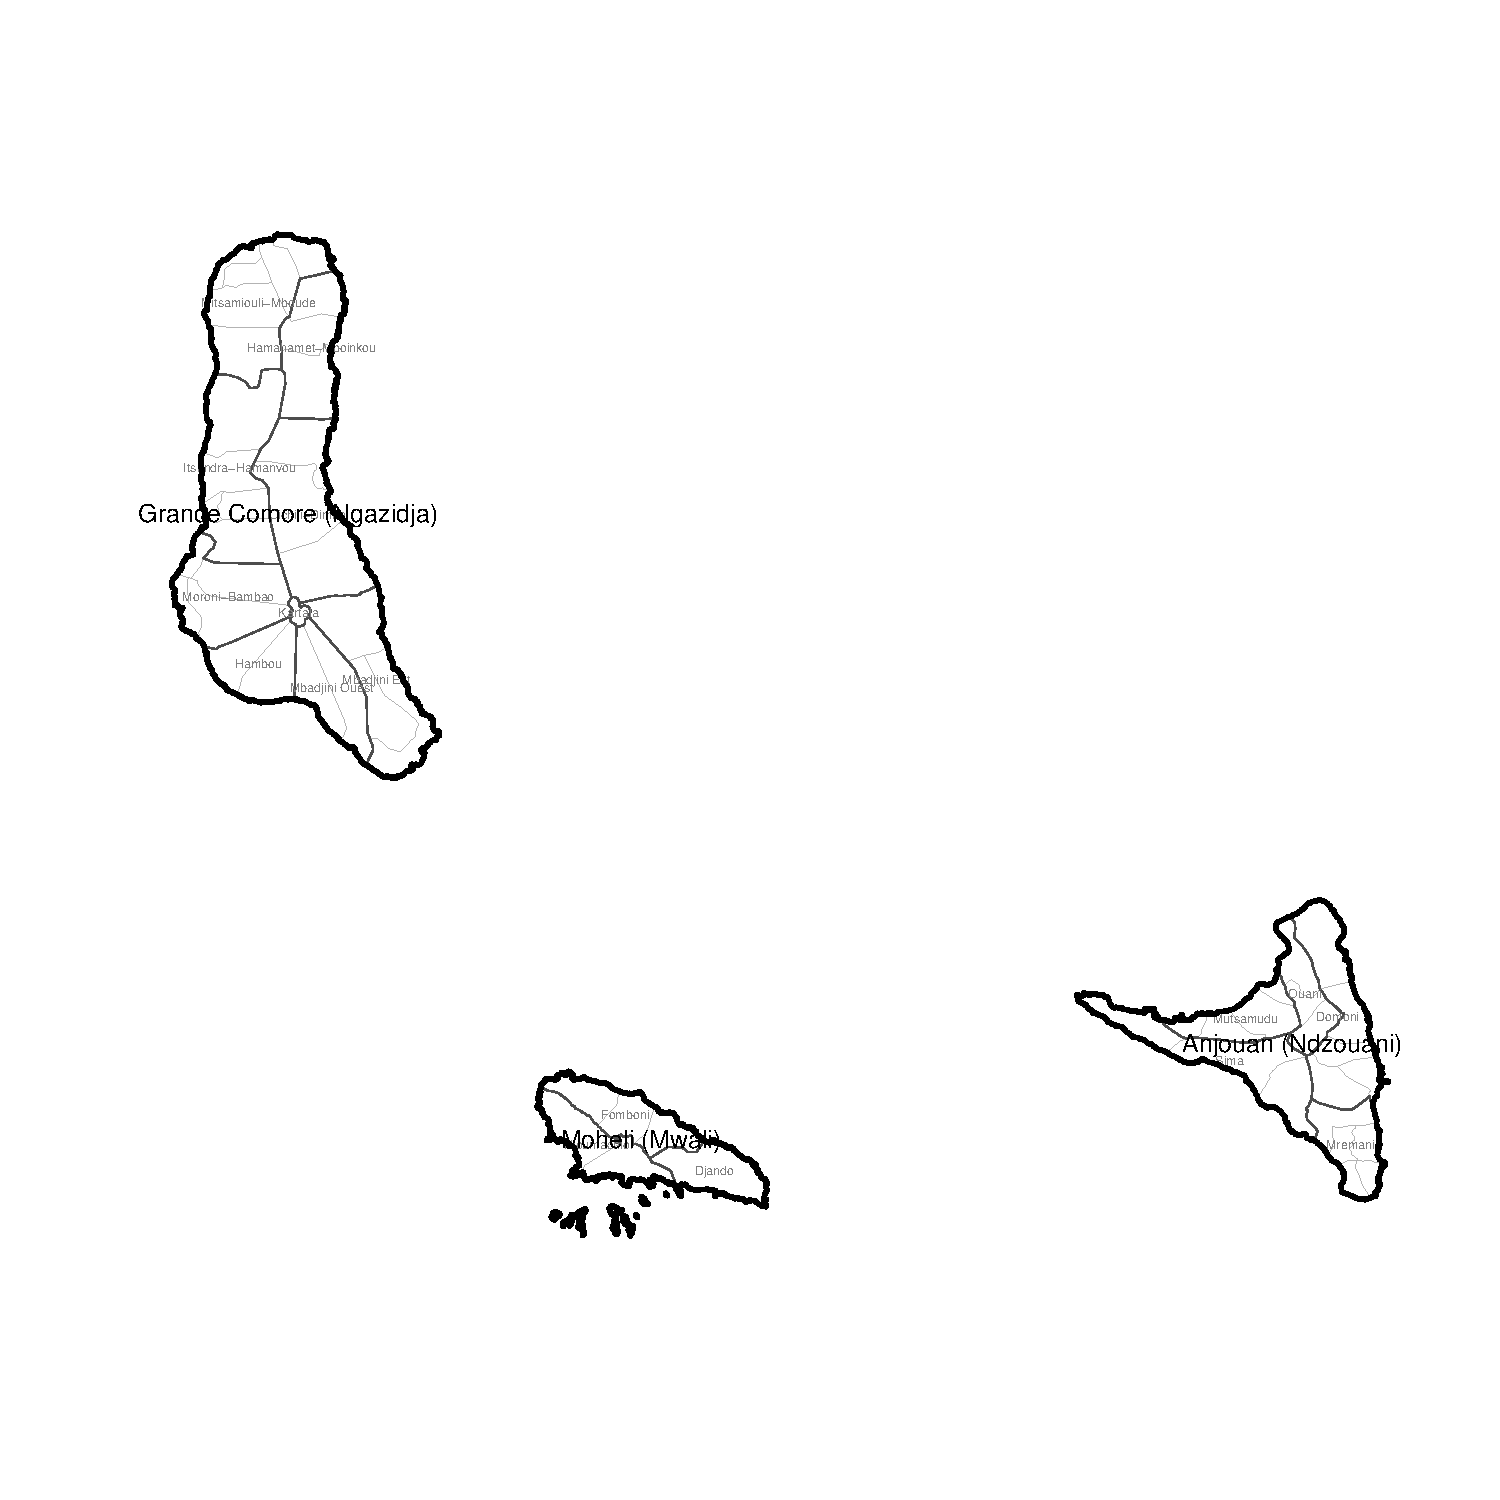
\includegraphics[width=0.9\linewidth]{comorosNotes_files/figure-latex/comorosMap-1} 

}

\caption{Map of Comoros}\label{fig:comorosMap}
\end{figure}

\hypertarget{proposed-indicators}{%
\section{Proposed indicators}\label{proposed-indicators}}

For purposes of health and nutrition programme planning for the Comoros, we propose the following reasonably comprehensive set of indicators as a starting point:

\begin{itemize}
\item
  Anthropometry:

  \begin{itemize}
  \item
    Prevalence of:

    \begin{itemize}
    \item
      Moderate and severe stunting (HAZ)
    \item
      Moderate and severe wasting (WHZ)
    \item
      Moderate and severe wasting (MUAC)
    \item
      Moderate and severe underweight (WAZ)
    \item
      Concurrent wasting and stunting (WHZ and HAZ)
    \item
      Combined GAM and combined SAM (MUAC, WHZ, oedema)
    \end{itemize}

    in children 6 to 59 months
  \item
    Prevalence of acute energy deficiency (MUAC) in mothers / carers
  \end{itemize}
\item
  Infant and child feeding index (ICFI) in children age 6 to 23 months extended using dietary diversity and meal frequency data in older children

  \begin{itemize}
  \tightlist
  \item
    ICFI provides a comprensive set of IYCF behavioural indicators and has been used in Demographic and Health Surveys (DHS) and is also frequently used in RAM surveys
  \end{itemize}
\item
  Dietary diversity scores for mothers (minimum dietary diversity for women or MDD-W) and children
\item
  Micronutrient consumption in mothers and children (from dietary diversity data)
\item
  14-day period prevalence by maternal recall of diarrhoea, acute respiratory infection (ARI), and fever of unknown origin (FUO) in children
\item
  Water, sanitation, and hygiene (WASH) indicators (Joint Monitoring Programme or JMP indicator set)
\item
  Expanded programme on immunisation (EPI) coverage
\item
  Vitamin A coverage
\item
  Deworming coverage
\item
  Bednet coverage (if appropriate to context)
\item
  IYCF counselling coverage (and recall of IYCF messages)
\item
  Coverage of community-based management of acute malnutrition (CMAM) screening services
\item
  Coverage of health extension services
\item
  Antenatal care (ANC) coverage indicators
\item
  Access to pre-school education (childen)
\item
  Maternal education
\item
  Multi-dimensional Poverty Index (MPI) or other poverty indices
\end{itemize}

Other indicators can be added. We prefer to use fully tested question sets and indicators and can advise on indicator selection. Let us know of indicators that you would like to add and we can provide specific guidance on whether these indicators will fit our approach and if not, what adaptations might be applied to these indicators to be fit for use with our approach.

\hypertarget{proposed-method}{%
\section{Proposed method}\label{proposed-method}}

Given the geography of the Comoros and with what we recommend as feasible and useful indicators for the purpose of health and nutrition programming in the country, we propose the Rapid Assessment Method or RAM. Applying RAM in the Comoros will include data collected and estimates made at prefecture (district) level using small sample surveys (e.g.~16 clusters of 12 mother-child pairs selected using simple to use and well-tested stratified spatial sampling methods). Surveys can be pooled (combined) to produce estimates at wider levels (e.g.~island and union level). Pooling of results will require prefecture level population data. Pooling of multiple RAM surveys can be seen as a ``poor man's MICS'' providing similar results quicker and at lower costs. Results can be mapped to prefecture level and above. RAM works with such small sample sizes (e.g. \(n ~ = ~ 192\)) because it uses modern and efficient indicators and computer intensive data analysis methods. All analysis is done using our free and open source ``workflow'' software.

\begin{figure}[H]

{\centering 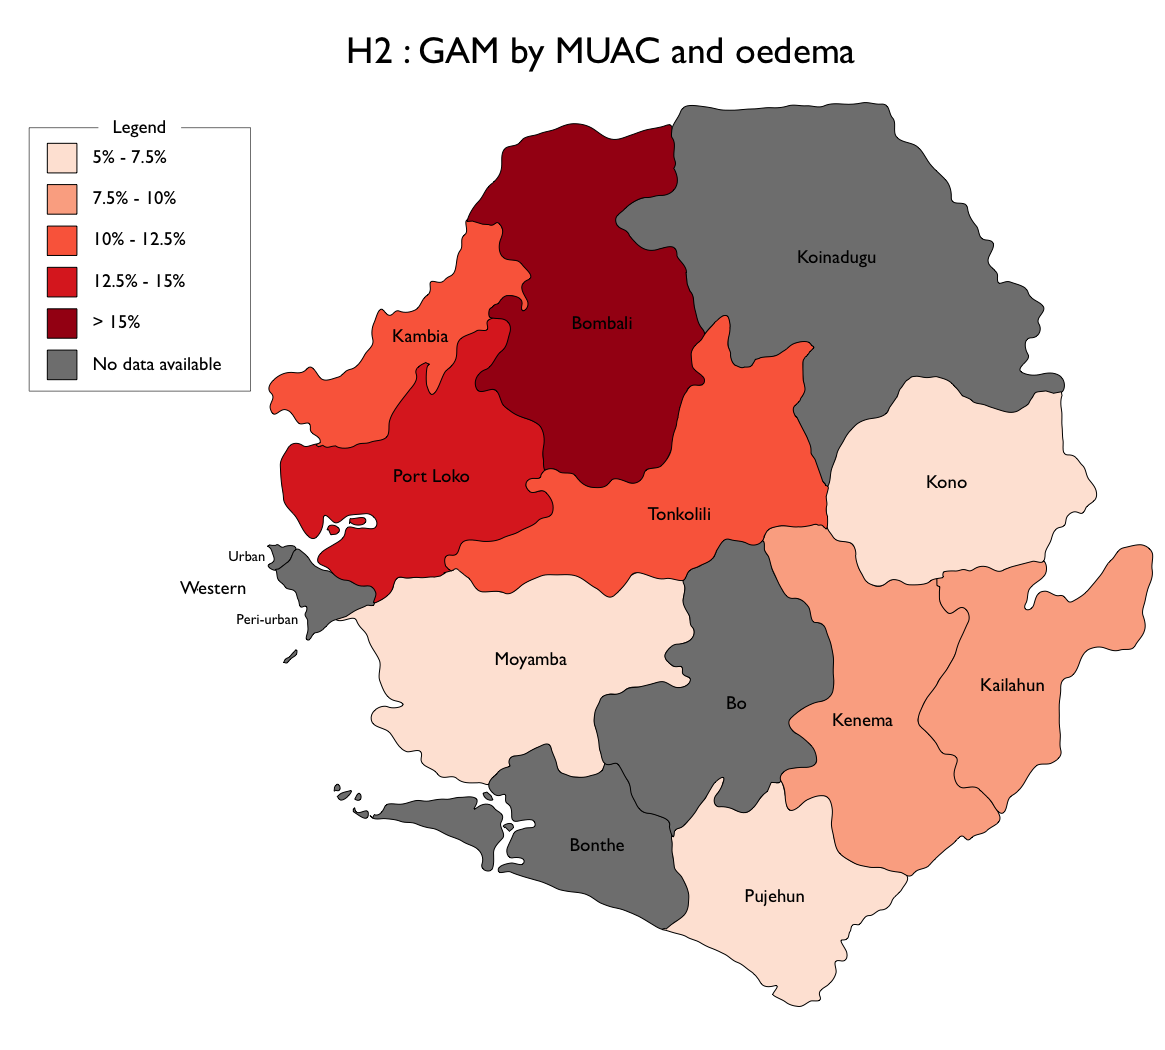
\includegraphics[width=0.7\linewidth]{figures/h2} 

}

\caption{Example results mapping from RAM surveys conducted in Sierra Leone by UNICEF}\label{fig:sampleResults11}
\end{figure}
\begin{figure}[H]

{\centering 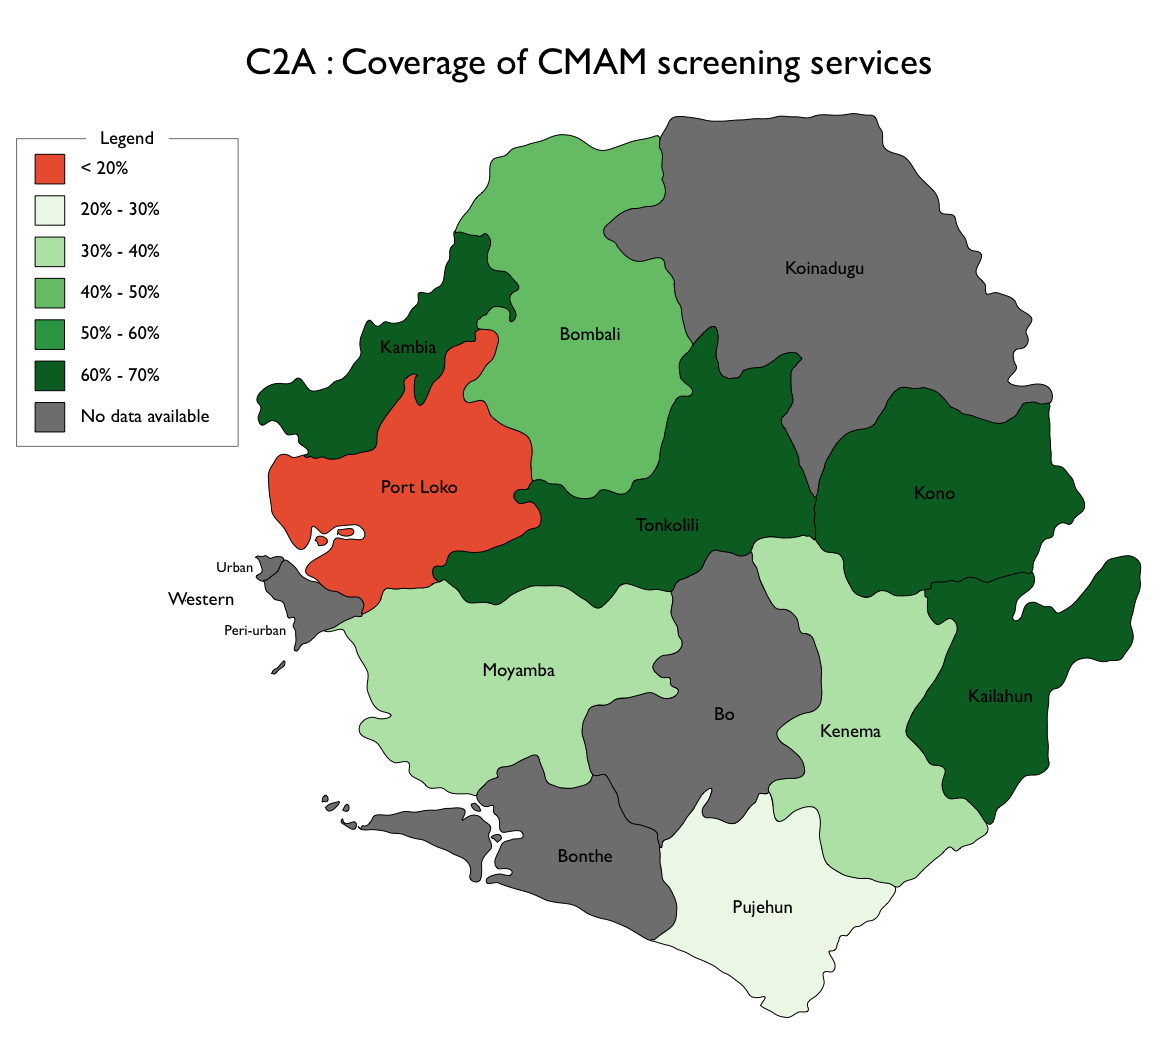
\includegraphics[width=0.7\linewidth]{figures/c2a} 

}

\caption{Example results mapping from RAM surveys conducted in Sierra Leone by UNICEF}\label{fig:sampleResults12}
\end{figure}
\begin{figure}[H]

{\centering 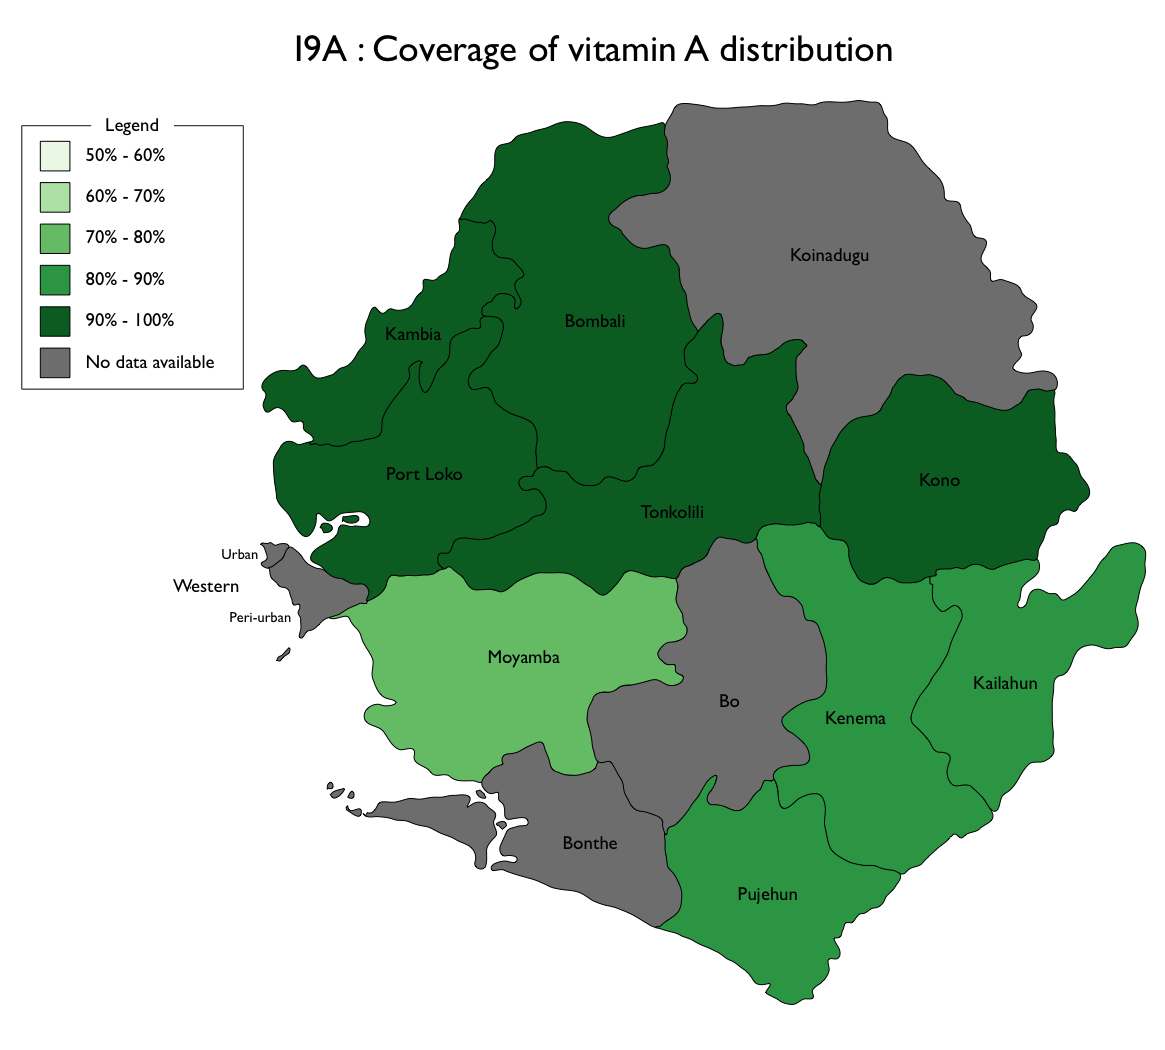
\includegraphics[width=0.7\linewidth]{figures/i9a} 

}

\caption{Example results mapping from RAM surveys conducted in Sierra Leone by UNICEF}\label{fig:sampleResults13}
\end{figure}

RAM has been used in Sierra Leone, Sudan, Bangladesh, Myanmar, Ethiopia, Tanzania, DRC, Malawi by UNICEF, MSF, GOAL, SC-US, Help-Age (RAM-OP), GAIN, and national governments.

\newpage

\hypertarget{implementation}{%
\section{Implementation}\label{implementation}}

We have experience rolling out RAM at the national level. We usually start by training many teams and supervisors in a single district. Teams can then return to home districts to complete further surveys. A typical district survey takes less than about 4 days to complete. Data-entry, data-analysis, and reporting usually takes only one additional day to complete. All data-analysis is done using our free and open source ``workflow'' software which we can easily customise to meet clients' needs. We can also provide training and support for survey and software customisation.

\begin{figure}

{\centering 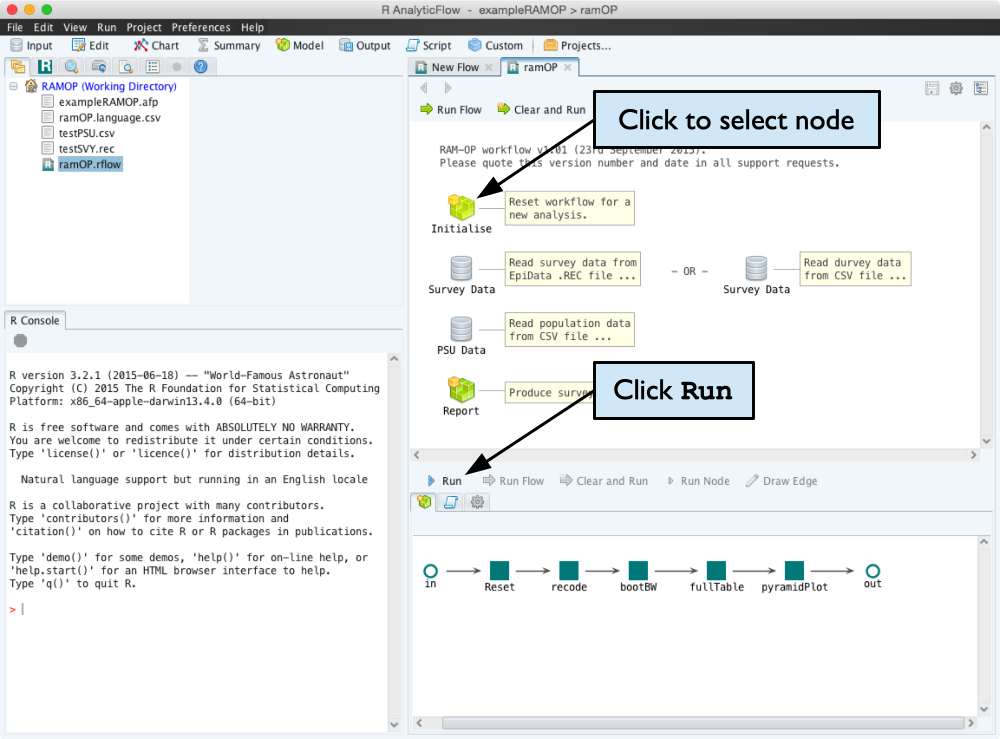
\includegraphics[width=13.89in]{figures/runWorkflowRAF} 

}

\caption{Example of a workflow system using RAnalyticFlow designed for RAM for Older People}\label{fig:workflow1}
\end{figure}

\begin{figure}[H]

{\centering 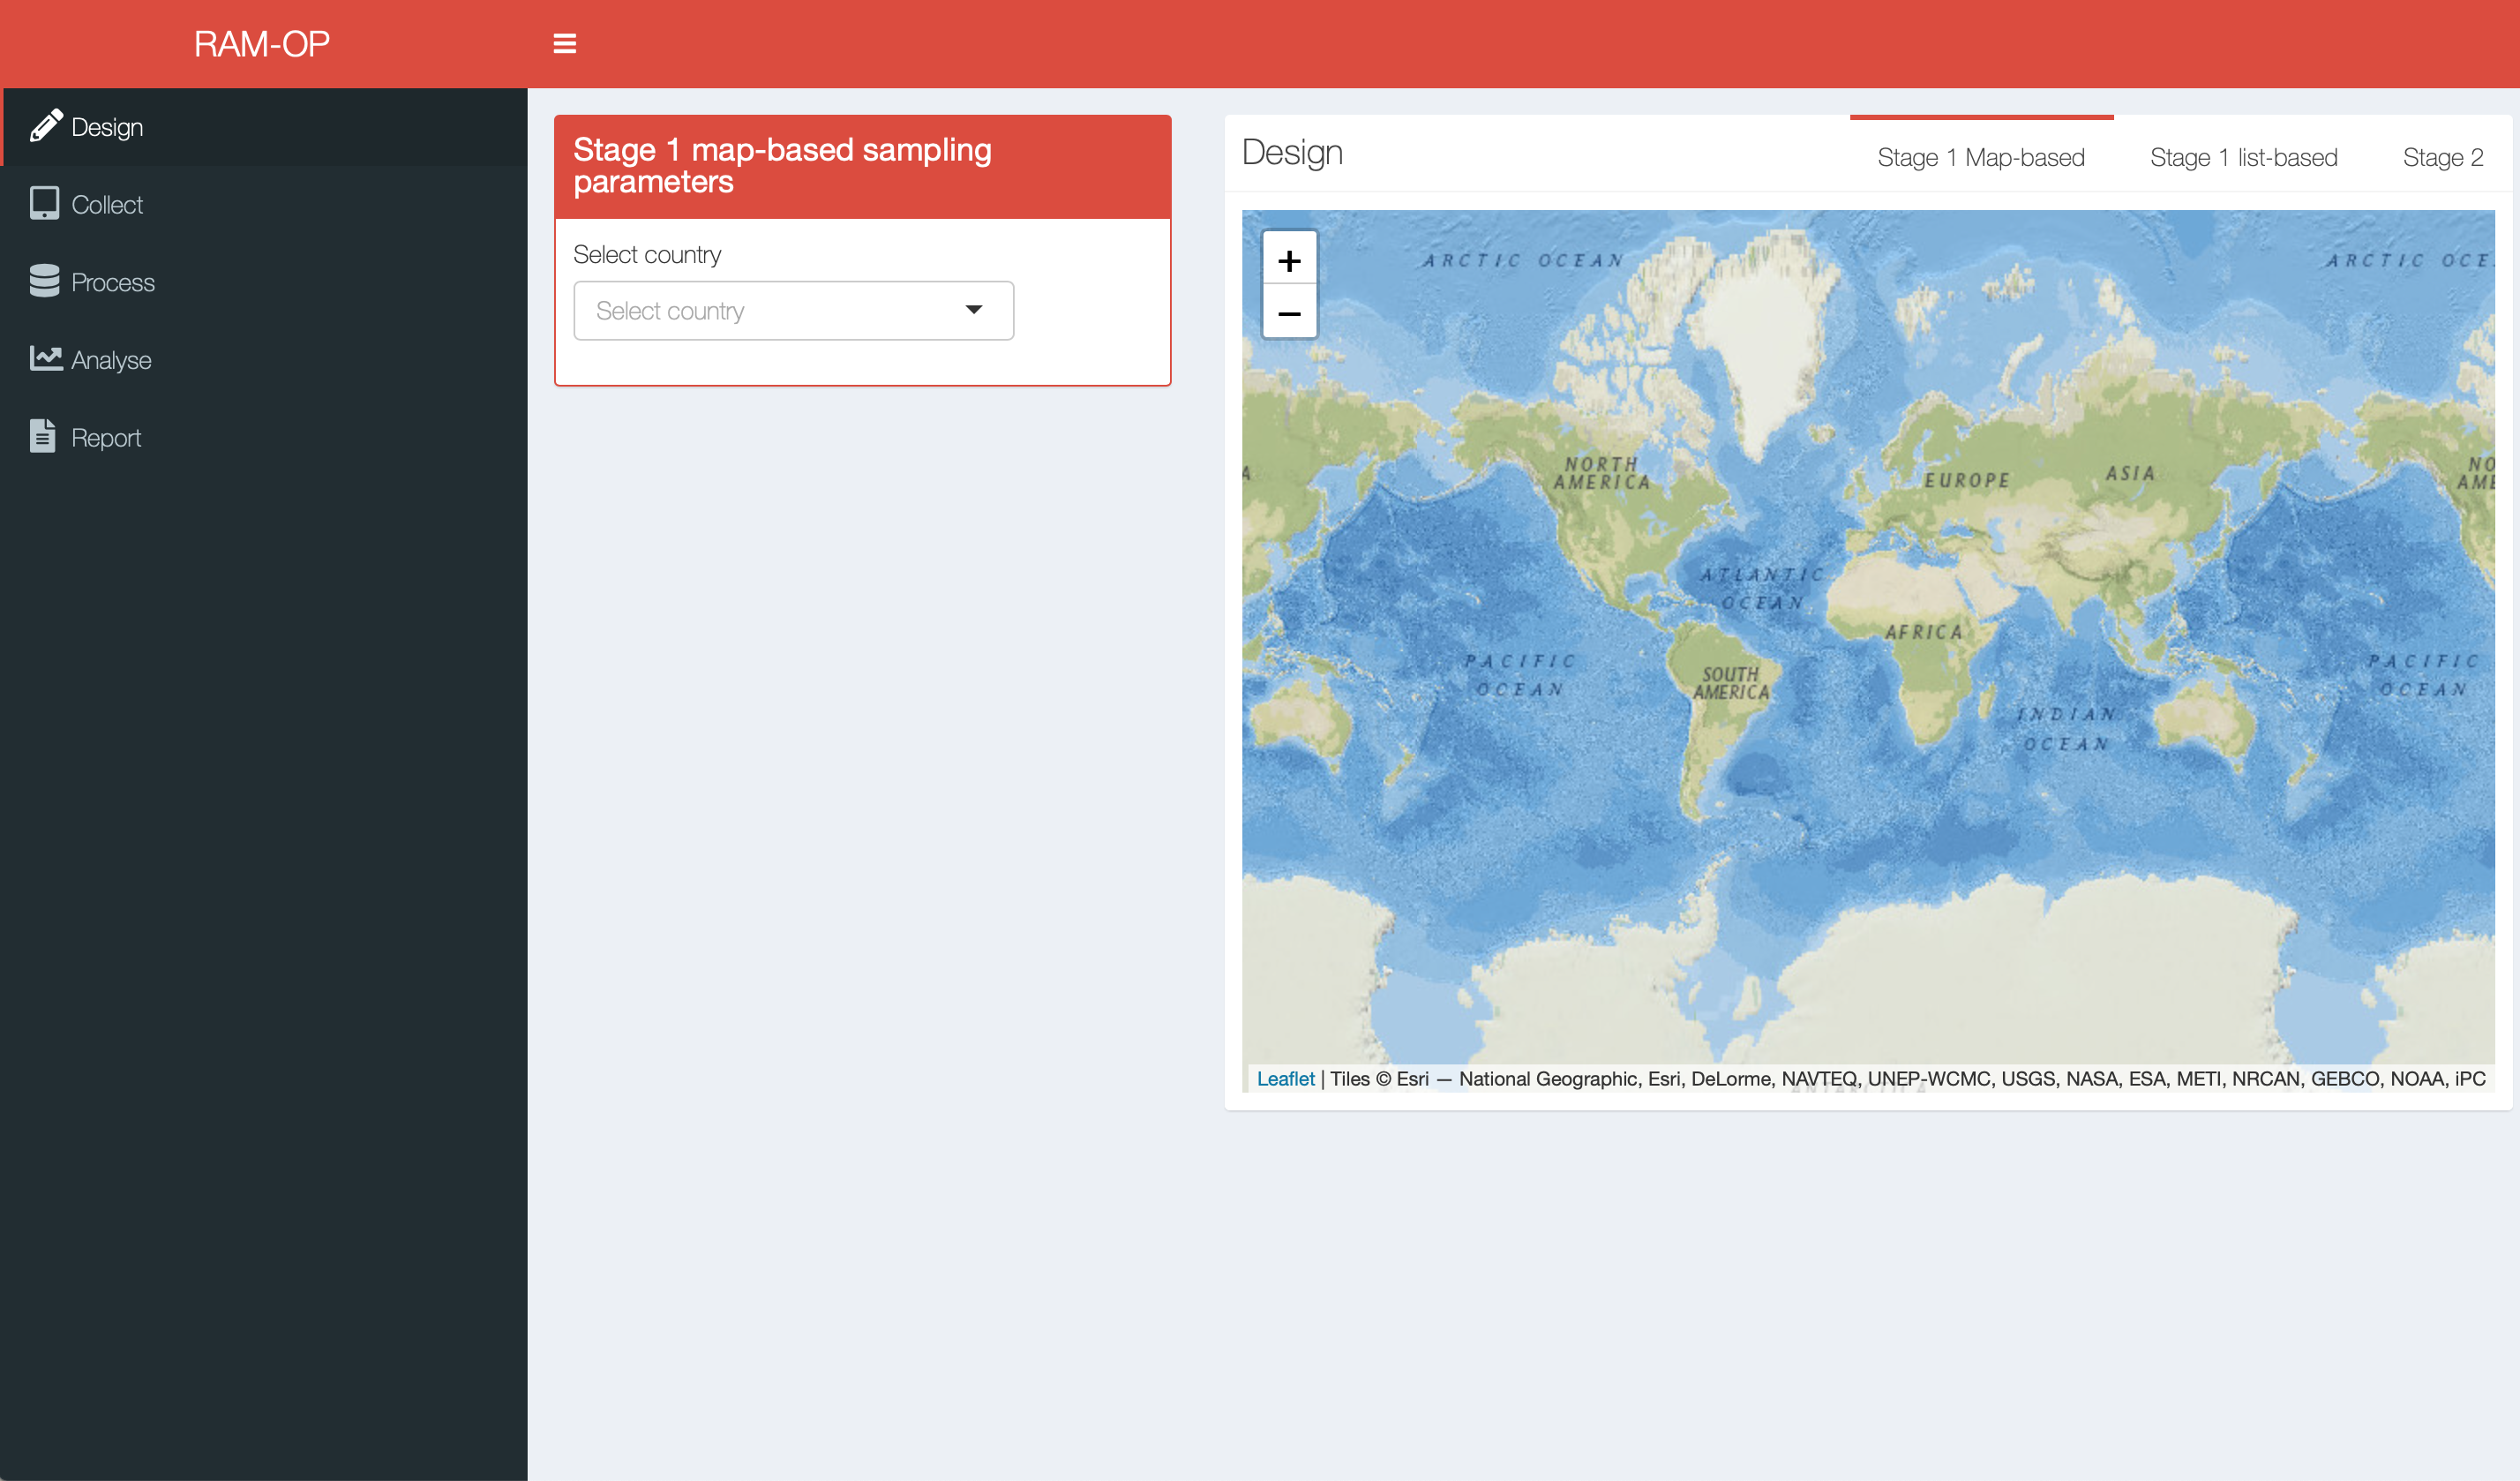
\includegraphics[width=0.9\linewidth]{figures/webWorkflow} 

}

\caption{Example of a web-based workflow system designed for RAM for Older People (https://rapidsurveys.shinyapps.io/ramOP)}\label{fig:workflow2}
\end{figure}

\bibliography{bibliography.bib}

\end{document}
